%----------------------------------------------------------------------------------------
%	PACKAGES AND OTHER DOCUMENT CONFIGURATIONS
%----------------------------------------------------------------------------------------

\documentclass[11pt]{article}
\usepackage{hyperref}
\input{structure.tex} % Include the file specifying the document structure and custom commands

%----------------------------------------------------------------------------------------
%	ASSIGNMENT INFORMATION
%----------------------------------------------------------------------------------------

% Required
\newcommand{\assignmentQuestionName}{} % The word to be used as a prefix to question numbers; example alternatives: Problem, Exercise
\newcommand{\assignmentClass}{Zero to ASIC} % Course/class
\newcommand{\assignmentTitle}{Analogue Design} % Assignment title or name
\newcommand{\assignmentAuthorName}{Thomas Parry} % Student name





% Optional (comment lines to remove)
%\newcommand{\assignmentClassInstructor}{Jones 10:30am} % Intructor name/time/description
%\newcommand{\assignmentDueDate}{Monday,\ January\ 24,\ 2019} % Due date

%----------------------------------------------------------------------------------------

\begin{document}

%----------------------------------------------------------------------------------------
%	TITLE PAGE
%----------------------------------------------------------------------------------------

\maketitle % Print the title page

\thispagestyle{empty} % Suppress headers and footers on the title page

\newpage


\section{Fundamentals of the MOSFET}

The MOSFET (Metal-Oxide Semiconductor Field Effect Transistor) is the fundamental building block of modern IC design.

\begin{figure}[h]
\centering{
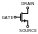
\includegraphics[scale=1.00]{diagrams/nmos.pdf}
}
\end{figure}

The MOSFET is a \textit{transconductance} device which translates a voltage between it's gate and source terminals to a current between the drain and source - assuming the device is biased correctly.

\subsection{The Saturation Region}

Most devices in a circuit will be operating in saturation where the following description of the current is given for a square-law device:

\begin{equation}
I_D = \frac{1}{2} \mu_n C_{ox} \frac{W}{L} {\left( V_{GS} - V_{TH} \right)}^2
\end{equation}

This can be simplified to:

\begin{equation}
I_D = K_n \frac{W}{L} {V_{OD}}^2
\end{equation}

\begin{equation}
given \; that: \;\;\; V_{DS} > V_{OD}
\end{equation}

The condition is very important, if you want your FET to work as expected you must ensure you have sufficient $V_{DS}$ headroom.  The value $V_{OD}$ is also more commonly called $V_{D_{SAT}}$ and is defined as the minimum drain voltage required to keep the device in saturation. Note that in sub-micron processes (like Skywater 130 nm) the statement that $V_{D_{SAT}} = V_{OD}$ is not fully accurate due to second order effects from device scaling.


\subsection{The Triode Region}

When there is insufficient drain-source voltage (by design or error) the device will work in the triode region where it approximates a voltage controlled resistor:

\begin{equation}
I_D = \mu_n C_{ox} \frac{W}{L} \left( (V_{GS} - V_{TH}) V_{DS} - \frac{V_{DS}^2}{2} \right)
\end{equation}

\subsection{The Cutoff Region}

When there is insufficient voltage across the gate-source terminals the device is 'off':

\begin{equation}
I_D = 0 \;\;\;\; given \; that: \;\; V_{GS} << V_{TH}
\end{equation}


\answer{Always know the region you expect your FET to operate and check that you have it correctly biased or all other assumptions are broken.}

\section{Basics of Transconductance Efficiency}

The transconductance is the amount of current in the drain per gate-source voltage.

\begin{equation}
i_d = g_m \cdot v_{gs}
\end{equation}

This simple diagram shows the most important concept of the FET: a voltage at the input is converted to an output current. This output current will later be converted by an impedance to another voltage.

\begin{figure}[h]
\centering{
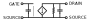
\includegraphics[scale=1.00]{diagrams/nmos_smallsignal.pdf}
}
\end{figure}


The transconductance can be expressed as a function of the bias current, giving the $g_m / I_d $ value. This value is related to how inverted the channel of the FET is - a measure of how 'turned on' the FET is. The measure of channel inversion is how many minority charge carriers have been attracted to the conductive channel between the source and drain.

\subsection{Transconductance Efficiency and Overdrive Voltage}

There is a relation to the overdrive voltage mentioned above, $V_{OD}$. The higher the $V_{OD}$, the more the FET is 'turned on', and therefore the more the FET channel is inverted, which leads to a \textit{lower} $g_m / I_d$. Conversly, a lower $V_{OD}$ turns on the FET less, and therefore the FET channel is less inverted, which leads to a \textit{higher} $g_m / I_d$.

\subsection{Realistic Values of Transconductance Efficiency}

There is a range of transconductance efficiencies that can be obtained in standard CMOS processes. It is reasonable to assume a maximum transconductance efficiency of 20 in design equations, although in some specific cases values of 25 can be reached. Typically a device will not be used below a transconductance efficiency of 4.

\subsection{Why Use Transconductance Efficiency?}

While transconductance efficiency, $g_m/I_d$, feels very abstract at first, its use lies in two factors.

\begin{enumerate}
  \item It gives a strong indication of the channel inversion.
  \item It allows quick calculation of circuit currents and other conditions.
\end{enumerate}

For example, if I have determined I will use a FET in weak inversion and I need $1 \; mS$ of transconductance, then I very simply know the required current of $50 \; \mu A$.

\answer{But how do we know what transconductance we should use for a given FET? We'll discuss this in the next section where I will talk about the relation of matching and noise to transconductance.}

\textbf{Further Reading (clickable)}

\hspace{1cm} \href{http://web02.gonzaga.edu/faculty/talarico/EE406/documents/gmid.pdf}{gm/ID - Based Design}

\hspace{1cm} \href{http://web.eecs.utk.edu/~bblalock/ece532/ece532_pres_ekv_bsim.pdf}{An Introduction to the EKV Model and a comparison of EKV to BSIM}

\end{document}
